\documentclass[tikz,border=4pt]{standalone}
\usepackage{amsmath}
\usetikzlibrary{patterns}
\begin{document}
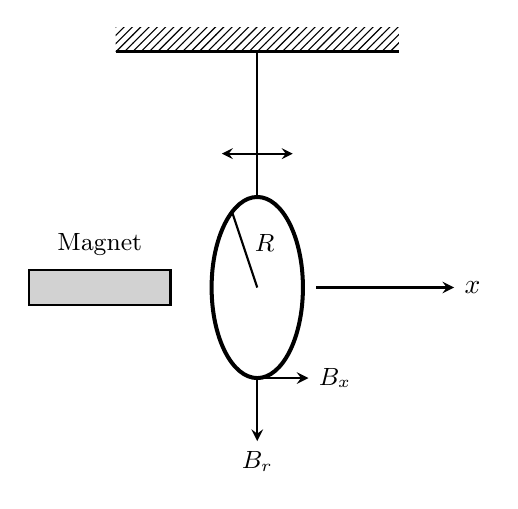
\begin{tikzpicture}[>=stealth, thick, scale=1.0]
  % Ceiling
  \fill[pattern=north east lines] (-1.8, 3.0) rectangle (1.8, 3.3);
  \draw[line width=1.0pt] (-1.8, 3.0) -- (1.8, 3.0);

  % Insulating wire
  \draw[line width=0.85pt] (0, 3.0) -- (0, 1.15);
  \draw[<->, line width=0.75pt] (-0.45, 1.7) -- (0.45, 1.7);

  % Bar magnet along x-axis on the left
  \fill[gray!35] (-2.9, -0.22) rectangle (-1.1, 0.22);
  \draw[line width=0.9pt] (-2.9, -0.22) rectangle (-1.1, 0.22);
  \node[above, font=\small] at (-2.0, 0.28) {$\mathrm{Magnet}$};

  % Conducting ring (ellipse in perspective) centered at (0, 0)
  \draw[line width=1.45pt] (0, 0) ellipse (0.58 and 1.15);
  \draw[line width=0.75pt] (0, 0) -- (-0.32, 0.96);
  \node[right, font=\small] at (-0.16, 0.56) {$R$};

  % x-axis extending to the right
  \draw[->, line width=0.85pt] (0.75, 0) -- (2.5, 0) node[right] {$x$};

  % Magnetic field components at bottom of ring (0, -1.15)
  \draw[->, line width=0.85pt] (0, -1.15) -- (0.65, -1.15) node[right, font=\small] {$B_x$};
  \draw[->, line width=0.85pt] (0, -1.15) -- (0, -1.95) node[below, font=\small] {$B_r$};
\end{tikzpicture}
\end{document}
